% !TeX root = ../main-english.tex
% !TeX spellcheck = en-US
% !TeX encoding = utf8
% -*- coding:utf-8 mod:LaTeX -*-

%This smart spell only works if no changes have been made to the chapter
%using the options proposed in preambel/chapterheads.tex.
\setchapterpreamble[u]{%
	\dictum[Ian Holmes, in an \href{https://twitter.com/ianholmes/status/288689712636493824}{\#overlyhonestmethods tweet}]{You can download our code from the URL supplied. Good luck downloading the only	postdoc who can get it to run, though.}
}


\chapter{Ensuring computational reproducibility across computational environments}
\label{chap:k3}

% from NISO: Beyond their potential to mitigate transparency and reproducibility issues, these practices provide important benefits for individual researchers by increasing exposure, reputation, chances of publication, number of citations, media attention, potential collaborations, and position and funding opportunities (Allen and Mehler, 2019; McKiernan et al., 2016; Nosek et al., 2022; Markowetz, 2015; Hunt, 2019).
Partially fueled by external incentives or requirements \citep{mckiernan2016open} \citep{dfg}, research curricula founded within the Open Science Movement \citep{munafo2017manifesto} \citep{poldrack2017scanning}, and a growing ecosystem of openly available infrastructure and tools \citep{NISO2022119623}, practices of publishing reproducibly are becoming more frequent.
Widespread sharing of code and data allows researchers to verify, reuse, and improve upon past work \citep{borghi2018data}.
Grass-roots movements such as Reprohack (\href{https://www.reprohack.org/}{www.reprohack.org}) or the ``Ten Years Reproducibility Challenge'' (\href{https://rescience.github.io/ten-years/}{rescience.github.io/ten-years}) train researchers to check published studies for reproducibility.
Consequently, attempts to reproduce previous studies often happen in different computational environments than those that originally created the results in question.
Ensuring computational reproducibility across computational environments is, however, a difficult technical challenge.
This following chapter outlines first its challenges, particularly in the field of neuroimaging, then its opportunities, and lastly an implementation to ensure computational reproducibility across computational environments.
Parts of this chapter were published as \citet{wagner2022fairly}: ``FAIRly big: A framework for computationally reproducible processing of large-scale data'' and are appropriately marked as such.


\section{The origins of reproducibility}

% from NISO: psychology (Open Science Collaboration, 2015; Klein et al., 2018), social sciences (Camerer et al., 2016, 2018), neuroimaging (Munafò et al., 2017; Botvinik-Nezer et al., 2020; Li et al., 2021), preclinical cancer biology research (Errington et al., 2021; Errington et al., 2021), and more (Hutson, 2018; Nissen et al., 2016; Serra-Garcia and Gneezy, 2021).
Over the past decade, interest in reproducibility has been fueled by salient failures to reconfirm published results in numerous fields, from psychology \citep{open2015estimating}, to biomedical imaging \citep{wagner202310}, to artificial intelligence \citep{hutson2018artificial}, or econonmics \citep{camerer2016evaluating}, often termed \textit{reproducibility crises}.
However, proposals to increase reproducibility, transparency, and robustness of science were made independently in various disciplines long before the current trend, in some cases dating back several centuries (maybe Robert Boyle, chemistry CITATION NEEDED).
Even the field of \textit{computational reproducibility} originated already more than 30 years ago in the field of seismology \citep{claerbout1992electronic} \citep{buckheit1995wavelab}, despite increased usage of the term in scientific literature only from 2015 onward (see \cref{fig:ngram}).
Consequently, the terminology around reproducibility has varied considerably over the years and across domains, and there is no universally agreed upon standardization of terminology in place yet \citep{barba2018terminologies}.
To disambiguate between several conflicting definitions of terms around reproducibility that are in active use, we shall define the terms used in this thesis as follows:

\subsubsection{Reproducibility}

Following the definition of \citet{peng2006}, \textit{reproducibility} refers to the practice of verifying a published result with the same methods and materials used by the original authors.

\subsubsection{Replicability}

\textit{Replicability}, on the other hand, refers to strengthening scientific evidence in favor of a result when ``multiple investigators [find similar results] using independent data, analytical methods, laboratories, and instruments''  \citep{peng2006}.

\subsubsection{Computational Reproducibility}

\textit{Computational reproducibility}, finally, matches the definition put forward in the 2019 report on ``Reproducibility and Replicability in Science'' by the National Academies of Science, Engineering and Medicine \citep{engineering2019reproducibility}: ``We define reproducibility to mean computational reproducibility – obtaining consistent computational results using the same input data, computational steps, methods, code, and conditions of analysis''.


\begin{figure}
	\centering
	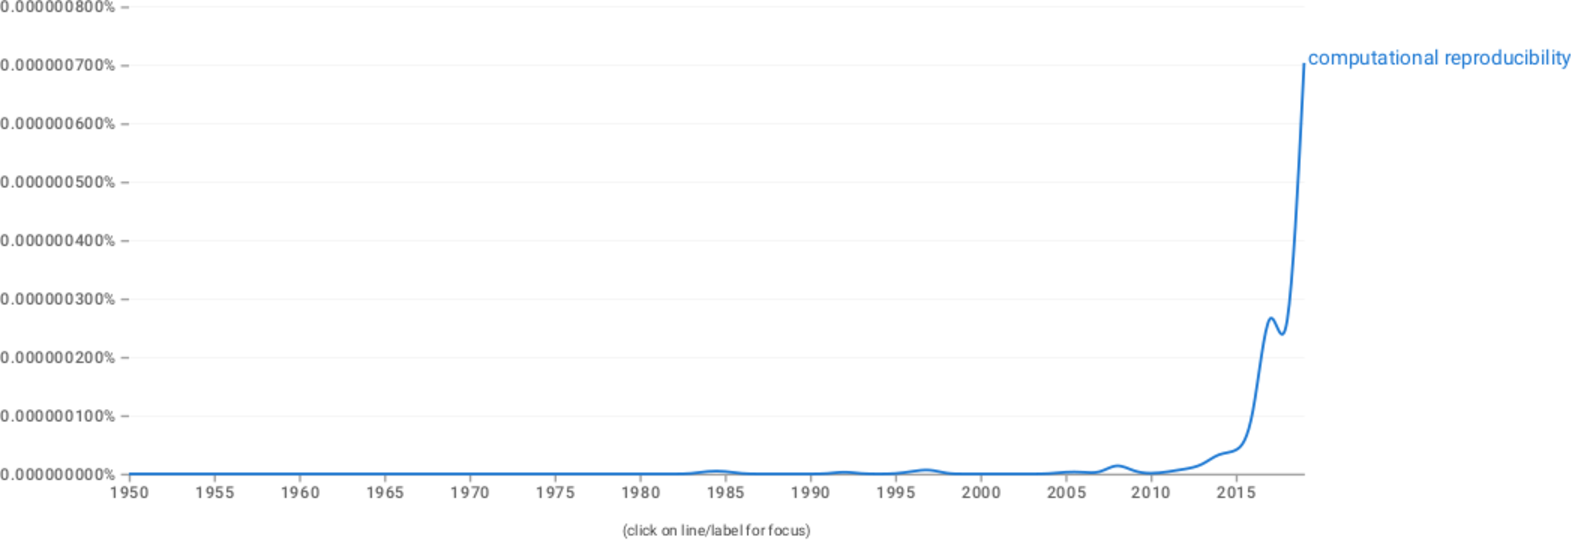
\includegraphics[width=\textwidth]{google_ngram_reproducibility_2023-05-08.pdf}
	\caption[Computational reproducibility in the literature]{Popularity of computational reproducibility: A chart of the frequencies of the n-gram ``computational reproducibility" (using yearly count, normalized be the numbers of publications in each year) in literature included in the English(2019) corpus of Google books. This graph has been created using the Google Ngram Viewer (\href{https://books.google.com/ngrams/info}{books.google.com/ngrams}) \citep{michel2011quantitative}}
	\label{fig:ngram}
\end{figure}


\subsection{``Everything matters'' for computational reproducibility in neuroimaging}

% maybe NARPS paper?`

The building blocks of research output extend to more than the files that constitute the actual research output, but also to all elements involved in its generation \citep{claerbout1992electronic}.
Consider different types of research output:
Raw data originates from acquisitions based on - potentially ongoing - experiments, raw data transformations, or data cleaning.
Processed data or results stem from computations with analysis code or software in specific versions on particular data.
And software, expressed in raw (code) or derived (transformed into executable) form, is created or used in specific computational environments, with compilers, underlying libraries, and systems in distinct versions.
Consequently, these building blocks play an integral part in the genesis of research outputs, and changes in these building blocks can translate to changes in the resulting research output.\\
The fact that different neuroimaging software tools can produce distinct results from the same data despite using similar conceptual methodology is well known \citep{bowring2019exploring}.
This has been attributed to implementation differences (CITATION NEEDED), software errors \citep{eklund2016cluster}, or analytic configurations.
For example, in task-based fMRI, \citet{li2021moving} found that the choice of output space or resolution can have a marked impact on variability between conceptually similar processing pipelines.
Moreover, surprising result variability can also occur when the same data is analyzed repeatedly with the same processing pipeline, but minor variations in parametrization. \citet{mueller2017commentary} reported that the choice of resampling resolution impacts alpha inflation, and \citet{li2021moving} identified the decision whether or not to include global signal regression as a major source of intra-pipeline variation.
But also different operating systems, or differences in versions of a singular software tool or operating system can result in different outcomes of the same analysis \citep{gronenschild2012effects} \citep{glatard2015reproducibility}.
Computational reproducibility across computing environments thus often remains elusive unless accounted for from the very start.
Therefore, in addition to ``Everything matters'',  \citet{kennedy2019everything} cued the phrase ``Reproducible by Design (as opposed to reproducibility as an afterthought)'' for conducting research in a way that makes computational reproducibility possible.
The next section highlights a number of strategies for this, and how reproducibility is tied to research data management.

% However, a growing number of studies suggest that differences in the implementation of these processing steps or how they are “glued together” can yield notably different outcomes. Studies systematically comparing specific preprocessing steps such as segmentation15, motion correction16, and registration17–19 have reported substantial variation in outputs generated across independently developed packages when applied to the same data. In the analysis of task fMRI data, end-to-end pipelines built using different software packages have been found to produce marked variation in the final results20–23. from https://www.biorxiv.org/content/10.1101/2021.12.01.470790v2.full


\section{Towards re-usable research objects}


The reusability of research objects has become a distinct characteristic of scientific practice as it allows for reproduction, verification, building up upon and extending existing work, evidence synthesis, and minimizing duplicate efforts in the advancement of science \citep{thanos2017research}.
With this, it maximizes the impact of the funding and work that resulted in the research output.
Therefore, it is considered the “ultimate goal” of the FAIR principles \citep{wilkinson2016fair}, and an explicit and central expectation in a variety of funding sources such as the Economic and Social Research Council (ESRC, UK), the European Research Council (ERC, EU), or the National Institutes of Health (NIH, US).

In the scope of the FAIR principles, reusability focuses on the ability of a human or a machine to decide if data are useful and usable in a particular context based on richly curated metadata.
This reusability requires trust \citep{bechhofer2010research}. Re-users must be able to audit the steps performed in an experiment or analysis in order to be convinced of the validity of the results or derivatives.
FAIR principle R1.2, ``(Meta)data are associated with detailed provenance'', refers to this.
In practice, however, the necessary standards and procedures for creating these metadata are not universally introduced,  incentivized, or required.
Where fully FAIR resources are still difficult or impractical to create, manual reproducibility typically provides this form of trust: for example when a new student checks if the previous findings that a their project builds up on still hold.



% curation needs to be pragmatic
Ideally, research data management creates reusable research outputs with little overhead, as an automatic byproduct of regular research activities.
If metadata curation efforts take place only after a research output has been generated, or are done by other people than the original creators, FAIRification can turn into a bureaucratic data governance effort with little immediately obvious benefits for the curator \citep{zehl2016handling}.

The term "reusable research object" was cued in a conceptual position paper by \citet{bechhofer2010research}, and defined as a ``container for a principled aggregation of resources, produced and consumed by common services and shareable within and across organisational boundaries. [...It] includes not only the data used, and methods employed to produce and analyse that data, but also the people involved in the investigation. An association with a dataset (or service, or result collection, or instrument) is now more than just a citation or reference to that dataset (or service or result collection). The association is rather a link to that dataset (or service or result collection) that can be explicitly followed or dereferenced providing access to the actual resource and thus enactment of the service, query or retrieval of data, and so on.''

% Detail how datalad adheres to these requirements.
In the following, I will argue why the \gls{rdm} features that DataLad provides fulfill these requirements, and how the DataLad dataset or its contents can be seen as a reusable research object.


\begin{figure}
	\centering
	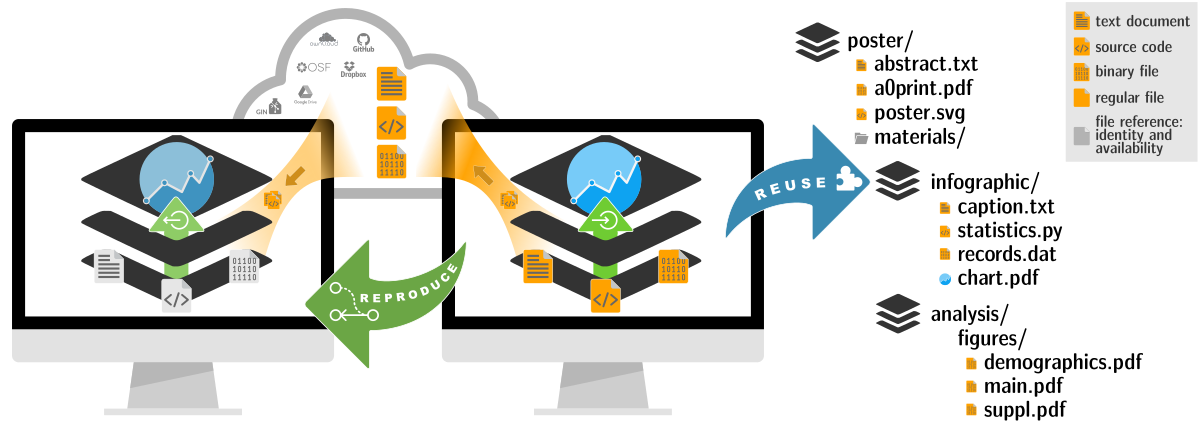
\includegraphics[width=.9\textwidth]{vamp.png}
	\caption[]{}
	\label{fig:ngram}
\end{figure}

In the spirit of this conceptual framework, the next section details a technical implementation and proof-of-concept analysis to create such reusable research objects as a byproduct of \gls{rdm} in analyses of any scale.



Those building blocks are integral information to retrace the genesis, reproduce, or trust research outputs (Kennedy et al., 2019), but they are rarely ever static.
Whatever created a given output evolves during usually incremental processes such as continuous quality control, acquisition, maintenance, or project revision.
However, changes in these building blocks will influence the resulting research output \citep{kennedy2019everything} 2019),\citep{glatard2015reproducibility}.
If it is not possible to precisely identify the foundational elements and everything involved in their creation, the reproducibility and reusability of research outputs and projects that use these objects is hence threatened \citep{kennedy2019everything}.
The information “I generated X from data Y with software Z” is insufficient for reproducibility and trustworthiness if Y exists in multiple versions or subsets, if different releases of Z have relevant implementation differences, or if Z behaves differently depending on the environment it is used in.
A prerequisite for identification is content tracking, such that changes in the evolution of digital files can be tagged and identified. If digital research objects are tracked, they can be accessed and used transparently in a uniquely identified version state.
This exhaustive identity registration removes ambiguity that arises if the files in question are not completely static.
Tracking can be applied with different levels of granularity, e.g., for each conceptually important step, or covering a complex transformation at once, but in both cases unambiguous identification of starting state, transformation, and end state is needed.
One way to track digital files is version control. If used appropriately, version control tools associate a unique identifier and basic provenance with each revision, and thus enable the identification of precise version states of digital files or collections of files. With other useful features such as built-in collaboration and the ability to save and revert changes, it also facilitates common scientific workflows, and has been increasingly adopted for research data management (RDM) in science \citep{nord2019towards} \citep{strupler2017reproducibility} \citep{bryan2018excuse} \citep{corti2019managing}.
While it is possible to exhaustively track all elements involved in a project with version control, industry use differs from RDM demands in science.
In industry contexts, it is primarily employed in software engineering for small-sized text files (source code). Science often works with large amounts of potentially sizable or binary files.
To exhaustively track all elements involved in a scientific project, large and binary files such as data and computational environments need to be versioned, too.
The concept of software containers - portable, light-weight software environments - make it possible to encapsulate computational environments as in-principle trackable elements, and a range of tools provide the ability to track even terabyte-sized and binary files.
Overall, version control is a well-established and reliable tool in industry and science. It can be employed at any point during a project, and yields a hands-on digital notebook of a project.
By extending its use beyond small-sized files to any digital research outputs and everything involved in its generation, version control can not only constitute established and beneficial research data management, but also lay the foundation for reusability by exhaustively tracking relevant digital elements and making them identifiable in precise versions.

From Donoho Buckheit 2015: Performance has everything to do with specifics: exactly what was done (which wavelets,
which coders, which detectors, which corpus of data) with exactly what parameters. In
this setting, publishing figures or results without the complete software environment could
be compared to a mathematician publishing an announcement of a mathematical theorem
without giving the proof. Waveleticians ought to publish their complete computational
environments


As highlighted in the Introduction, digital research outputs are the by- or end-products of scientific studies or analyses, from code, software, raw data or processed data, to analysis results or papers.

\pagebreak

\section{FAIRly big: A framework for computationally reproducible processing of large-scale data}

% role of sample size for reproducible results: \citep{li2021moving}

%  \citep{li2021moving} "highlight the reality that as the test-retest reliability approaches optimal levels for laboratory measurement, pipeline implementation differences will impose an inherent upper bound on the agreement of preprocessed data. These findings also underscore that 10 minutes of data, which has been common in the field until at least recent years, are insufficient for producing results that are reliable enough to reveal substantive pipeline-related variation."


\begin{figure}
	\centering
	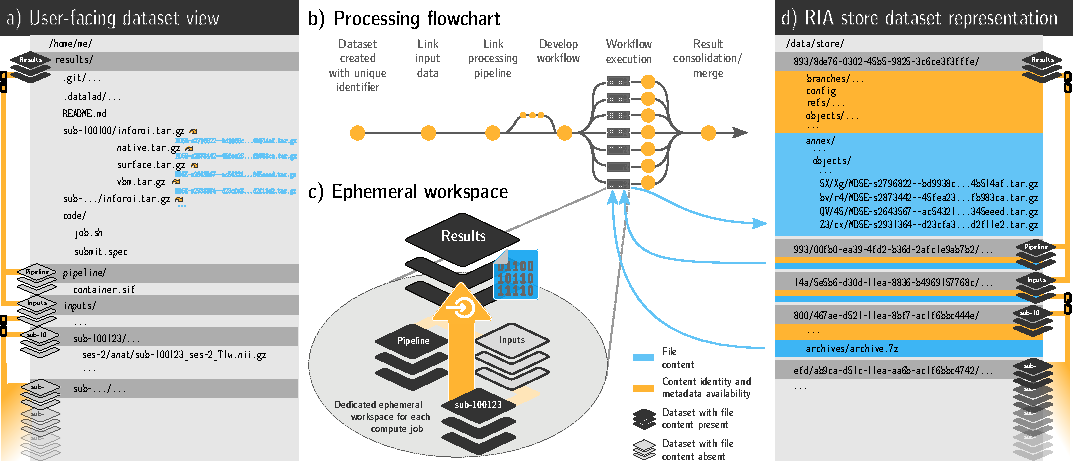
\includegraphics[width=\textwidth]{ukbworkflow_simplified.pdf}
	\caption[]{}
	\label{fig:ngram}
\end{figure}

\begin{figure}
	\centering
	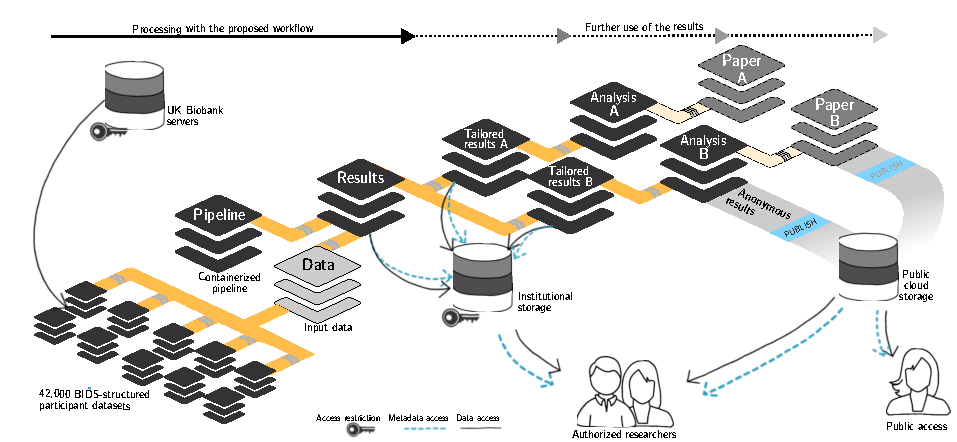
\includegraphics[width=\textwidth]{ukb_datasets.pdf}
	\caption[]{}
	\label{fig:ngram}
\end{figure}

\begin{figure}
	\centering
	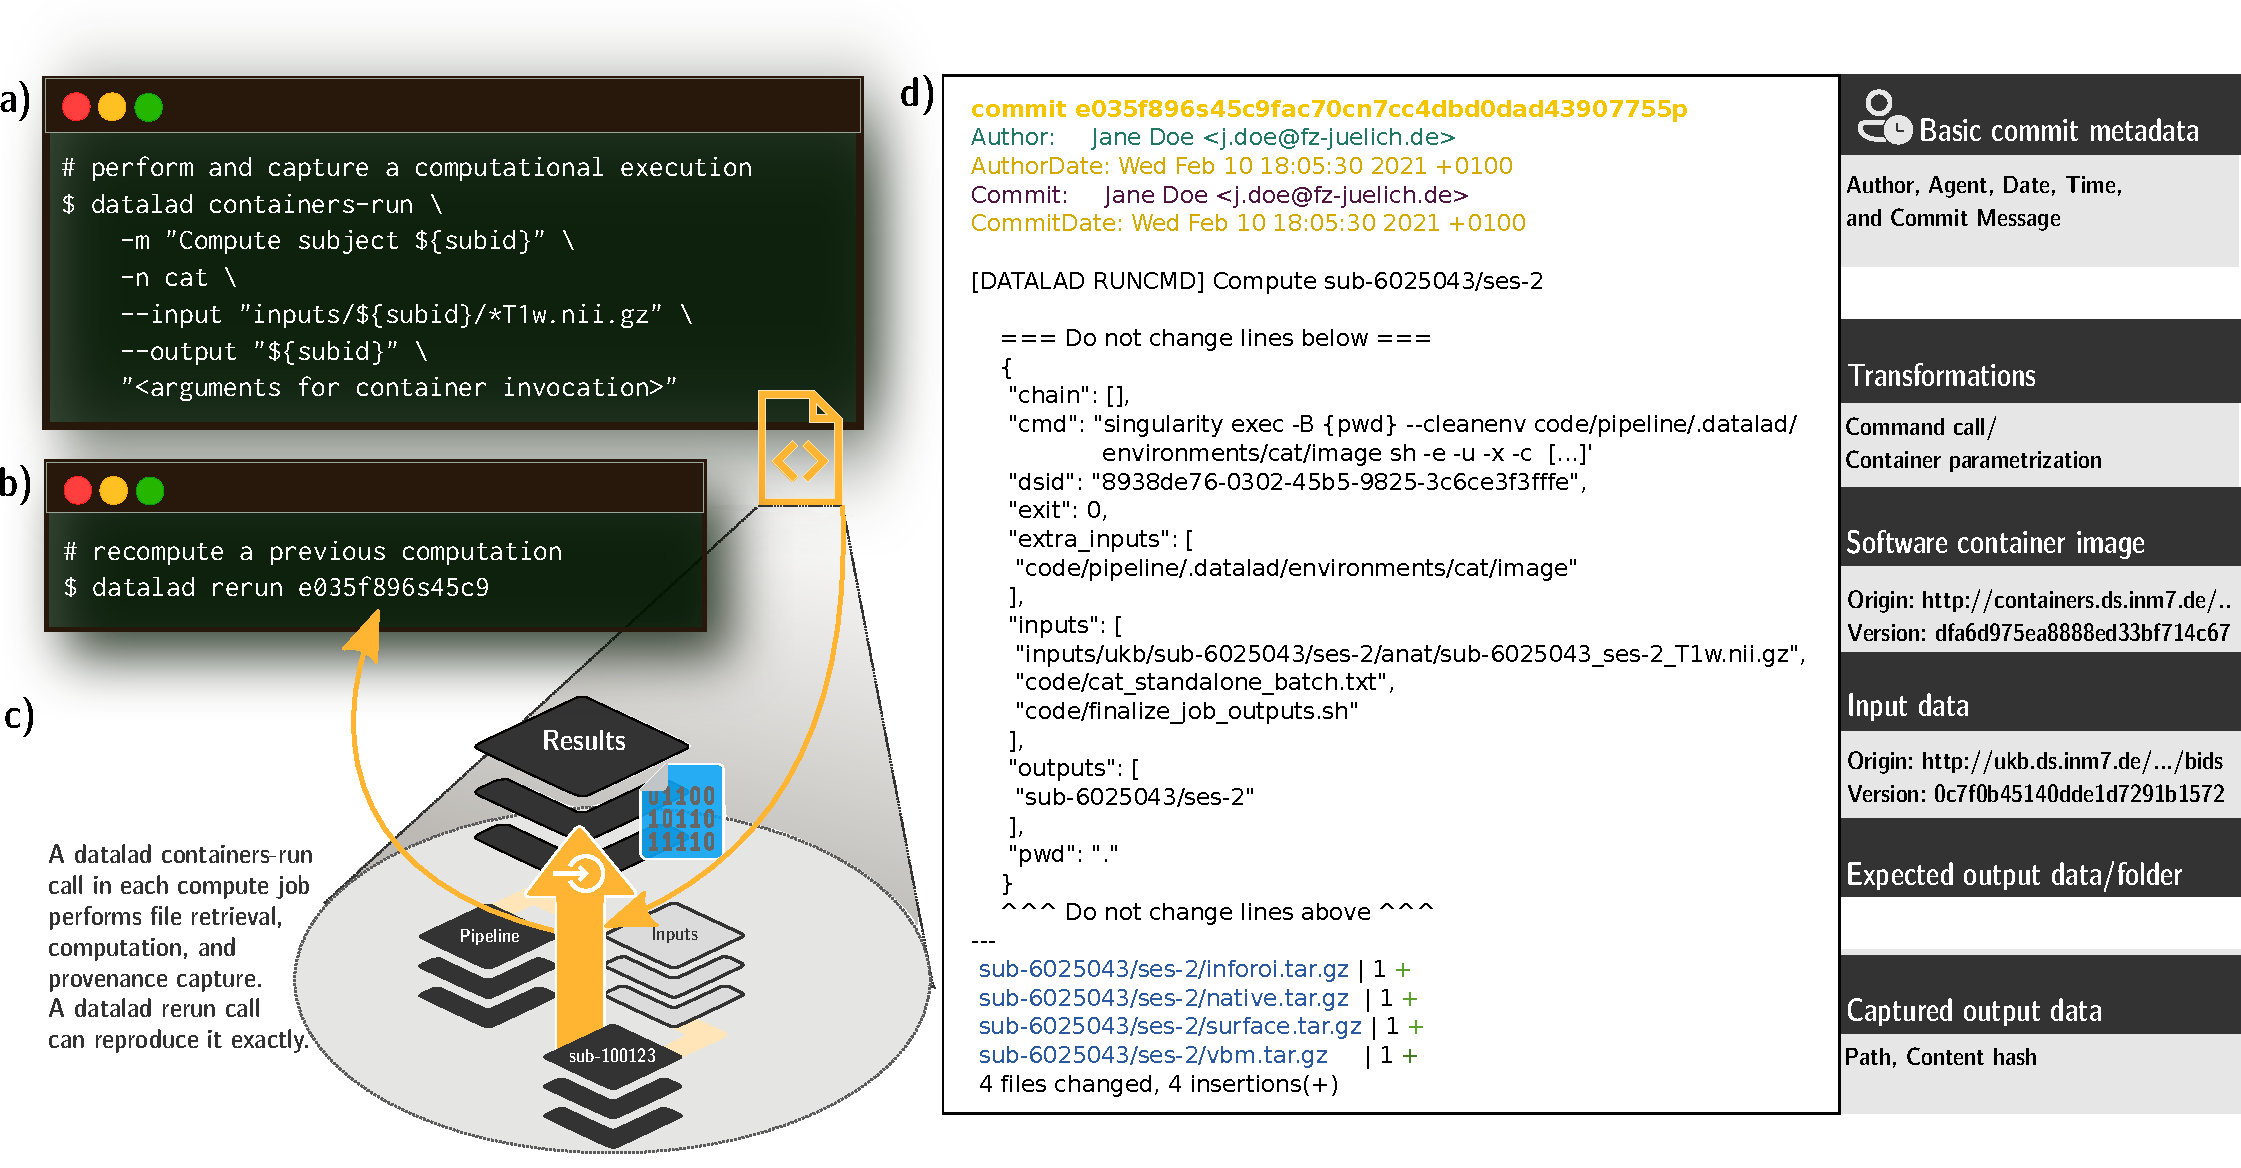
\includegraphics[width=\textwidth]{coarsemetadata.pdf}
	\caption[]{}
	\label{fig:ngram}
\end{figure}

% on re-analyzing the pipeline, cite li2021moving: "we demonstrated the role that pipeline replication can play as a means of exploring analytic variation and assessing the robustness of findings. To this end, we leveraged and extended the flexibility of C-PAC to replicate non-MATLAB dependent minimal processing pipelines (ABCD-BIDS, CCS, fMRIPrep-LTS) in a single platform"


\pagebreak